\documentclass[12pt]{article}

\usepackage{enumitem}
\usepackage{hyperref}
\usepackage{amsthm}
\usepackage{tikz}
\usepackage{amsmath}
\usepackage{color}
\usepackage{bm}
\usepackage{array}

\newtheoremstyle{parenbold} % Name
  {2\parskip}           % Space above
  {}                    % Space below
  {}  % Body font
  {}                    % Indent amount
  {\bfseries}           % Theorem head font
  {}                    % Punctuation after theorem head
  { }                 % Space after theorem head
  {\thmnumber{#2 }\thmname{#1.\newline}\thmnote{\bfseries{#3} |}} % Theorem head spec
  
\makeatletter
\g@addto@macro\bfseries{\boldmath}
\makeatother

\theoremstyle{parenbold}
\newtheorem{definition}{Definition}[section]

\newtheorem{exmp}{Example}[section]

\newtheorem{lemma}{Lemma}[section]

\newtheorem{theorem}{Theorem}[section]

\title{C\&O URA Spring 2017}
\author{Zach Dockstader}

\begin{document}
\maketitle

\tableofcontents

\section{Inertia Bounds}

\subsection{Introduction on Inertia Bounds}
\theoremstyle{definition}
\begin{definition}[Independent Set]
An independent set is a set of vertices belonging to a graph in which no two vertices are adjacent.
\end{definition}
\begin{exmp}
Consider the following graph:\\
\\
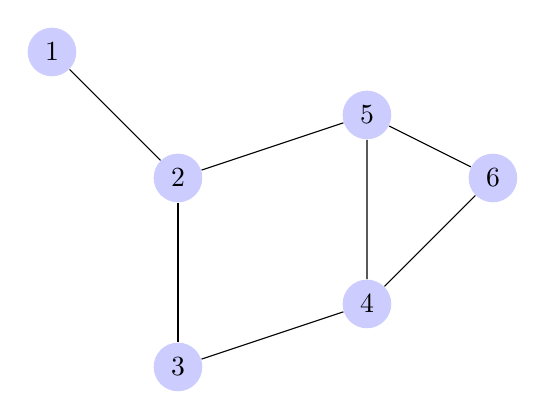
\begin{tikzpicture}
[scale=.8,every node/.style={circle,fill=blue!20}]
\node (n1) at (1,10) {1};
\node (n2) at (3,8) {2};
\node (n3) at (3,5) {3};
\node (n4) at (6,6) {4};
\node (n5) at (6,9) {5};
\node (n6) at (8,8) {6};
\foreach \from/\to in {n1/n2,n2/n3,n2/n5,n3/n4,n5/n4,n5/n6,n4/n6}
\draw (\from) -- (\to);
\end{tikzpicture}

An example of an independent set in this graph is:\\
\\
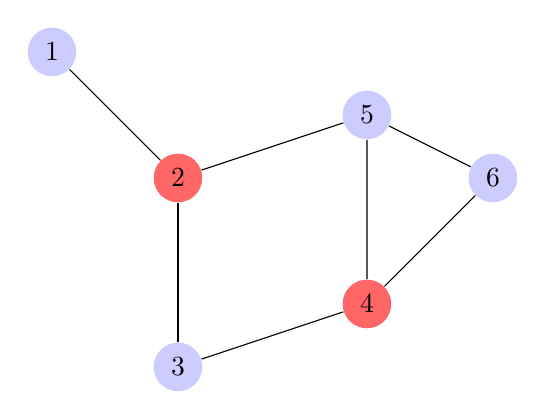
\begin{tikzpicture}
[scale=.8,every node/.style={circle,fill=blue!20}]
\node (n1) at (1,10) {1};
\node[fill=red!60] (n2) at (3,8) {2};
\node (n3) at (3,5) {3};
\node[fill=red!60] (n4) at (6,6) {4};
\node (n5) at (6,9) {5};
\node (n6) at (8,8) {6};
\foreach \from/\to in {n1/n2,n2/n3,n2/n5,n3/n4,n5/n4,n5/n6,n4/n6}
\draw (\from) -- (\to);
\end{tikzpicture}

However, often the independent set we are most interested in finding is the largest one:\\
\\
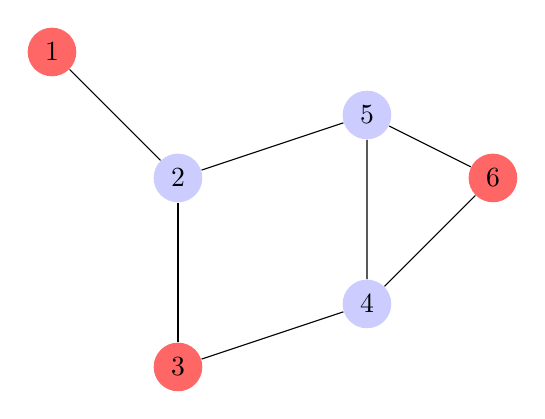
\begin{tikzpicture}
[scale=.8,every node/.style={circle,fill=blue!20}]
\node[fill=red!60] (n1) at (1,10) {1};
\node (n2) at (3,8) {2};
\node[fill=red!60] (n3) at (3,5) {3};
\node (n4) at (6,6) {4};
\node (n5) at (6,9) {5};
\node[fill=red!60] (n6) at (8,8) {6};
\foreach \from/\to in {n1/n2,n2/n3,n2/n5,n3/n4,n5/n4,n5/n6,n4/n6}
\draw (\from) -- (\to);
\end{tikzpicture}
\end{exmp}
\begin{definition}[Independence Number]
The independence number of a graph $G$, denoted $\alpha(G)$, is the size of the largest independent set of $G$.
\end{definition}

\begin{definition}[Weight Matrix]
The weight matrix of a graph $G$, is a matrix defined by:

\begin{equation}
    W_{i,j} = 
    \begin{cases}
        c_{i,j} & \mbox{if $v_i$ and $v_j$ are adjacent} \\
        0 & \mbox{otherwise}
    \end{cases}
\end{equation}
with $v_i$ a vertice of $G$ and $c_{i,j}$, a constant.

The weight matrix of a graph, is identical to an adjacency matrix, except where there was a 1 in the matrix at entry $A_{i,j}$ if vertices $v_i$ and $v_j$ were adjacent, there is now a constant indicating a weighting for the edge between $v_i$ and $v_j$.

\end{definition}

For any graph $G$, there exists a bound on $\alpha(G)$, known as the Cvetkovi\'c bound (also referred to as the Interia Bound). This bound provides a relationship between $\alpha(G)$ and the number of positive, negative, and zero eigenvalues of the weight matrix, $W$, associated with $G$. The Cvetkovi\'c bound of $G$, is:

\begin{equation}
\alpha(G) \leq \min\{|G| - n_+(W),|G|-n_-(W)\}
\end{equation}

Where $n_+(W)$ and $n_-(W)$ denote the number of positive and negative eigenvalues of $W$, respectively.

To prove this, we first need to introduce a result that comes from the Eigenvalue Interlacing Theorem:

\begin{theorem}[Corollary of Eigenvalue Interlacing Theorem]
\label{interlacing}
Let $A$ be an $n\times n$ real symmetric matrix with eigenvalues $\lambda_1 \geq \lambda_2 \geq \ldots \geq \lambda_n$ and let $C$ be a $k\times k$ principal submatrix of $A$ with eigenvalues $\tau_1 \geq \tau_2 \geq \ldots \geq \tau_k$. Then $\lambda_i \geq \tau_i$ for all $i$ $\in \{1,\ldots ,k\}$. \cite{sinkovic2016graph}
\end{theorem}

\begin{definition}[Principal Submatrix]
The principal submatrix of an $n\times n$ matrix $A$ is the submatrix obtained where if $row_i$ is excluded in the submatrix, then $column_i$ is excluded as well. Note that all principal submatrices of a weight matrix $W$, correspond to an induced subgraph in the graph represented by $W$.
\end{definition}

\begin{exmp}
The following is an example of a principal submatrix in relation to graph theory.

Consider the following graph:

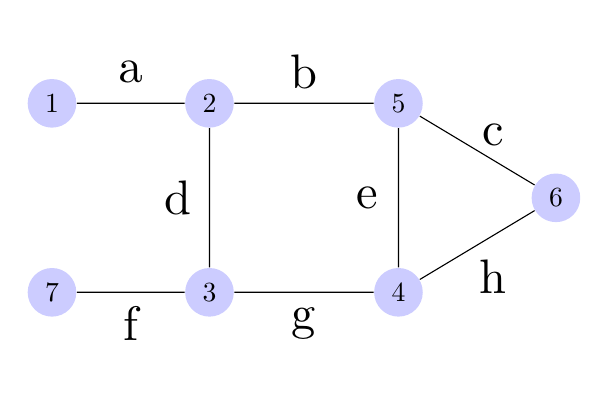
\begin{tikzpicture}
[scale=.8,every node/.style={circle,fill=blue!20}]
\node[scale=1.75,fill=white] (a) at (2.75,9.5) {a};
\node[scale=1.75,fill=white] (b) at (5.5,9.5) {b};
\node[scale=1.75,fill=white] (c) at (8.5,8.5) {c};
\node[scale=1.75,fill=white] (d) at (3.5,7.5) {d};
\node[scale=1.75,fill=white] (e) at (6.5,7.5) {e};
\node[scale=1.75,fill=white] (f) at (2.75,5.5) {f};
\node[scale=1.75,fill=white] (g) at (5.5,5.5) {g};
\node[scale=1.75,fill=white] (h) at (8.5,6.25) {h};
\node (n1) at (1.5,9) {1};
\node (n2) at (4,9) {2};
\node (n3) at (4,6) {3};
\node (n4) at (7,6) {4};
\node (n5) at (7,9) {5};
\node (n6) at (9.5,7.5) {6};
\node (n7) at (1.5,6) {7};
\foreach \from/\to in {n1/n2,n2/n3,n2/n5,n3/n4,n5/n4,n5/n6,n4/n6,n3/n7}
\draw (\from) -- (\to);
\end{tikzpicture}

and corresponding weight matrix:

$
\begin{bmatrix}
0 & a & 0 & 0 & 0 & 0 & 0 \\
a & 0 & d & 0 & b & 0 & 0 \\
0 & d & 0 & g & 0 & 0 & f \\
0 & 0 & g & 0 & e & h & 0 \\
0 & b & 0 & e & 0 & c & 0 \\
0 & 0 & 0 & h & c & 0 & 0 \\
0 & 0 & f & 0 & 0 & 0 & 0 \\
\end{bmatrix}
$
\\
\\
We can see the following principal submatrix and corresponding induced subgraph:

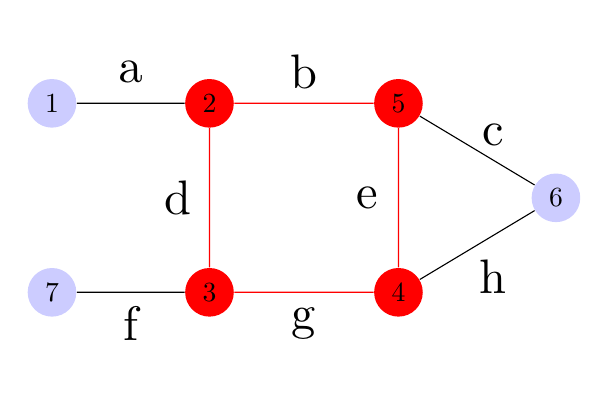
\begin{tikzpicture}
[scale=.8,every node/.style={circle,fill=blue!20}]
\node[scale=1.75,fill=white] (a) at (2.75,9.5) {a};
\node[scale=1.75,fill=white] (b) at (5.5,9.5) {b};
\node[scale=1.75,fill=white] (c) at (8.5,8.5) {c};
\node[scale=1.75,fill=white] (d) at (3.5,7.5) {d};
\node[scale=1.75,fill=white] (e) at (6.5,7.5) {e};
\node[scale=1.75,fill=white] (f) at (2.75,5.5) {f};
\node[scale=1.75,fill=white] (g) at (5.5,5.5) {g};
\node[scale=1.75,fill=white] (h) at (8.5,6.25) {h};
\node (n1) at (1.5,9) {1};
\node[fill=red] (n2) at (4,9) {2};
\node[fill=red] (n3) at (4,6) {3};
\node[fill=red] (n4) at (7,6) {4};
\node[fill=red] (n5) at (7,9) {5};
\node (n6) at (9.5,7.5) {6};
\node (n7) at (1.5,6) {7};
\foreach \from/\to in {n1/n2,n5/n6,n4/n6,n3/n7}
\draw (\from) -- (\to);
\draw[red](n2) -- (n5);
\draw[red](n2) -- (n3);
\draw[red](n3) -- (n4);
\draw[red](n4) -- (n5);
\end{tikzpicture}

$
\begin{bmatrix}
0 & a & 0 & 0 & 0 & 0 & 0 \\
a & \color{red}0 & \color{red}d & \color{red}0 & \color{red}b & 0 & 0 \\
0 & \color{red}d & \color{red}0 & \color{red}g & \color{red}0 & 0 & f \\
0 & \color{red}0 & \color{red}g & \color{red}0 & \color{red}e & h & 0 \\
0 & \color{red}b & \color{red}0 & \color{red}e & \color{red}0 & c & 0 \\
0 & 0 & 0 & h & c & 0 & 0 \\
0 & 0 & f & 0 & 0 & 0 & 0 \\
\end{bmatrix}
$
\\

As well, we see the following principal submatrix of an independent set of the graph:

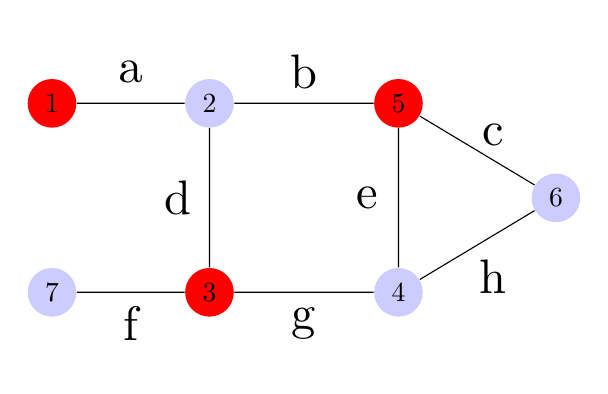
\begin{tikzpicture}
[scale=.8,every node/.style={circle,fill=blue!20}]
\node[scale=1.75,fill=white] (a) at (2.75,9.5) {a};
\node[scale=1.75,fill=white] (b) at (5.5,9.5) {b};
\node[scale=1.75,fill=white] (c) at (8.5,8.5) {c};
\node[scale=1.75,fill=white] (d) at (3.5,7.5) {d};
\node[scale=1.75,fill=white] (e) at (6.5,7.5) {e};
\node[scale=1.75,fill=white] (f) at (2.75,5.5) {f};
\node[scale=1.75,fill=white] (g) at (5.5,5.5) {g};
\node[scale=1.75,fill=white] (h) at (8.5,6.25) {h};
\node[fill=red] (n1) at (1.5,9) {1};
\node (n2) at (4,9) {2};
\node[fill=red] (n3) at (4,6) {3};
\node (n4) at (7,6) {4};
\node[fill=red] (n5) at (7,9) {5};
\node (n6) at (9.5,7.5) {6};
\node (n7) at (1.5,6) {7};
\foreach \from/\to in {n1/n2,n2/n3,n2/n5,n3/n4,n5/n4,n5/n6,n4/n6,n3/n7}
\draw (\from) -- (\to);
\end{tikzpicture}

$
\begin{bmatrix}
\color{red}0 & a & \color{red}0 & 0 & \color{red}0 & 0 & 0 \\
a & 0 & d & 0 & b & 0 & 0 \\
\color{red}0 & d & \color{red}0 & g & \color{red}0 & 0 & f \\
0 & 0 & g & 0 & e & h & 0 \\
\color{red}0 & b & \color{red}0 & e & \color{red}0 & c & 0 \\
0 & 0 & 0 & h & c & 0 & 0 \\
0 & 0 & f & 0 & 0 & 0 & 0 \\
\end{bmatrix}
$
\\
\end{exmp}

Now to prove the Cvetkovi\'c Bound:

\begin{theorem}[Cvetkovi\'c Bound]
Let $G$ be a graph on n vertices, and $W$ be the weight matrix of $G$. Then the following inequality holds:
\begin{equation}
\alpha(G) \leq \min\{|G| - n_+(W),|G|-n_-(W)\}
\end{equation}
\end{theorem}

\begin{proof}\footnote{Interesting Graphs and their Colourings, unpublished lecture notes C. Godsil (2004)}
Let $H$ be the subgraph of $G$ formed by the vertices in an independent set of size s. Then $H$ is an induced subgraph of $G$ and all eigenvalues of the principal submatrix $W(H)$ are 0 since the principal submatrix will just be a zero matrix. Let $\lambda_i$ denote the $i$th largest eigenvalue of $W$ and $\tau_i$ denote the $i$th larest eigenvalue of $W(H)$. Now, by interlacing, we have,
\begin{equation}
\lambda_i \geq \tau_i = 0 \text{ for all i } \in \{1,\ldots ,s\}
\end{equation}

and so 
\begin{equation}
n - n_-(W) = n_+(W) + n_0(W) \geq s
\end{equation}
Also, note that by negating $W$, the positive eigenvalues become negative eigenvalues and vice versa. Thus,
\begin{equation}
n - n_+(W) = n - n_-(-W),
\end{equation}
However, the principal submatrix corresponding to $H$ in $-W$ is still the zero matrix and thus has all zero eigenvalues. Thus, by interlacing, we get a similar result as above, 
\begin{equation}
n - n_+(W) = n - n_-(-W) = n_+(-W) + n_0(-W) \geq s
\end{equation}

Therefore, both $n - n_+(W)$ and $n - n_-(W)$ are greater than or equal to s. Since s is the size of the idependent set, we can see that letting s = $\alpha(G)$, we get:

\begin{equation}
\alpha(G) \leq \min\{|G| - n_+(W),|G|-n_-(W)\}
\end{equation}

\end{proof}

\subsection{Graphs with Tight Inertia Bounds}

\subsubsection{Perfect Graphs}

\begin{definition}[Chromatic Number]
The chromatic number of a graph, $\chi(G)$, is the minimum number of colours needed in a proper colouring of G. \cite{elzinga2007minimum}
\end{definition}

\begin{exmp}
Consider the following graph:
\\

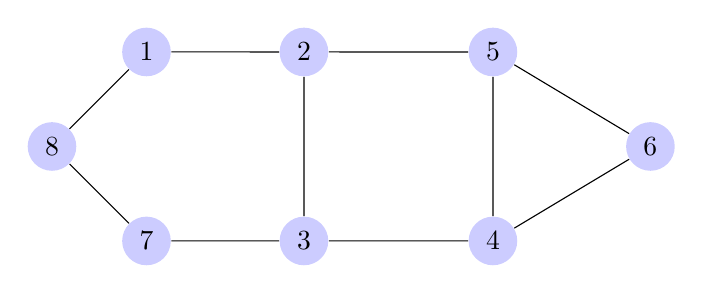
\begin{tikzpicture}
[scale=.8,every node/.style={circle,fill=blue!20}]
\node (n1) at (1.5,9) {1};
\node (n2) at (4,9) {2};
\node (n3) at (4,6) {3};
\node (n4) at (7,6) {4};
\node (n5) at (7,9) {5};
\node (n6) at (9.5,7.5) {6};
\node (n7) at (1.5,6) {7};
\node (n8) at (0,7.5) {8};
\foreach \from/\to in {n1/n2,n2/n3,n2/n5,n3/n4,n5/n4,n5/n6,n4/n6,n3/n7,n7/n8,n1/n8}
\draw (\from) -- (\to);
\end{tikzpicture}

An example of a colouring would be:
\\

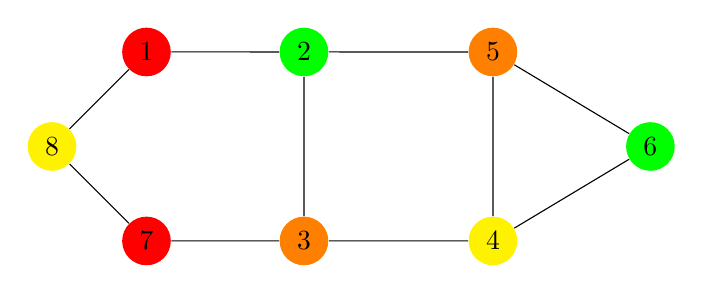
\begin{tikzpicture}
[scale=.8,every node/.style={circle,fill=blue!20}]
\node[fill=red] (n1) at (1.5,9) {1};
\node[fill=green] (n2) at (4,9) {2};
\node[fill=orange] (n3) at (4,6) {3};
\node[fill=yellow] (n4) at (7,6) {4};
\node[fill=orange] (n5) at (7,9) {5};
\node[fill=green] (n6) at (9.5,7.5) {6};
\node[fill=red] (n7) at (1.5,6) {7};
\node[fill=yellow] (n8) at (0,7.5) {8};
\foreach \from/\to in {n1/n2,n2/n3,n2/n5,n3/n4,n5/n4,n5/n6,n4/n6,n3/n7,n7/n8,n1/n8}
\draw (\from) -- (\to);
\end{tikzpicture}

However, $\chi(G)$ for this graph is 3:
\\

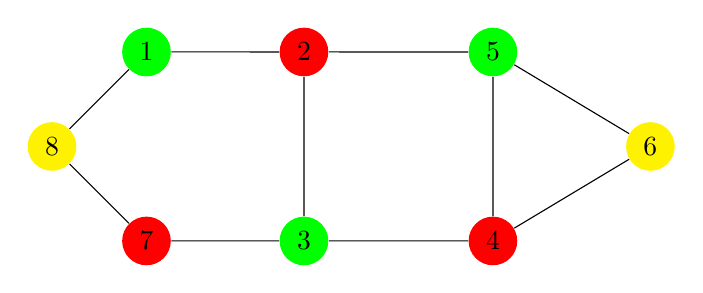
\begin{tikzpicture}
[scale=.8,every node/.style={circle,fill=blue!20}]
\node[fill=green] (n1) at (1.5,9) {1};
\node[fill=red] (n2) at (4,9) {2};
\node[fill=green] (n3) at (4,6) {3};
\node[fill=red] (n4) at (7,6) {4};
\node[fill=green] (n5) at (7,9) {5};
\node[fill=yellow] (n6) at (9.5,7.5) {6};
\node[fill=red] (n7) at (1.5,6) {7};
\node[fill=yellow] (n8) at (0,7.5) {8};
\foreach \from/\to in {n1/n2,n2/n3,n2/n5,n3/n4,n5/n4,n5/n6,n4/n6,n3/n7,n7/n8,n1/n8}
\draw (\from) -- (\to);
\end{tikzpicture}

\end{exmp}

\begin{definition}[Clique]
An m-clique in a graph is a complete subgraph on m vertices. \cite{elzinga2007minimum}

The clique number, $\omega(G)$, is the number of vertices in a maximum clique of $G$.

\end{definition}

\begin{definition}[Clique Cover]
A Clique Cover of the vertex set $V(G)$ of a graph $G$ is a set of cliques $C$, such that each vertex is in at least one clique in $C$. 

The clique cover number, $\theta(G)$ is the minimum number of cliques needed in a clique cover of $G$. \cite{elzinga2007minimum}

\end{definition}

\begin{exmp}
Consider the following graph:
\\
\\
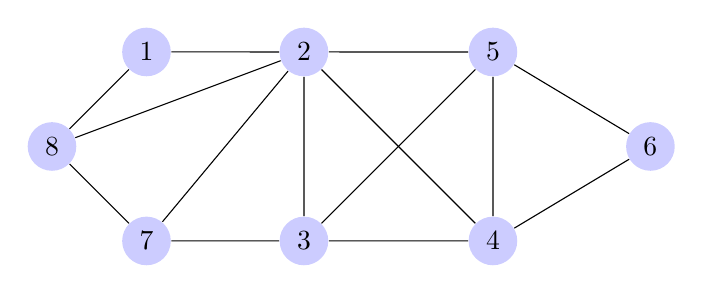
\begin{tikzpicture}
[scale=.8,every node/.style={circle,fill=blue!20}]
\node (n1) at (1.5,9) {1};
\node (n2) at (4,9) {2};
\node (n3) at (4,6) {3};
\node (n4) at (7,6) {4};
\node (n5) at (7,9) {5};
\node (n6) at (9.5,7.5) {6};
\node (n7) at (1.5,6) {7};
\node (n8) at (0,7.5) {8};
\foreach \from/\to in {n1/n2,n2/n3,n2/n5,n3/n4,n5/n4,n5/n6,n4/n6,n3/n7,n7/n8,n1/n8,n2/n4,n3/n5,n2/n7,n2/n8}
\draw (\from) -- (\to);
\end{tikzpicture}

A possible clique covering is:
\\
\\
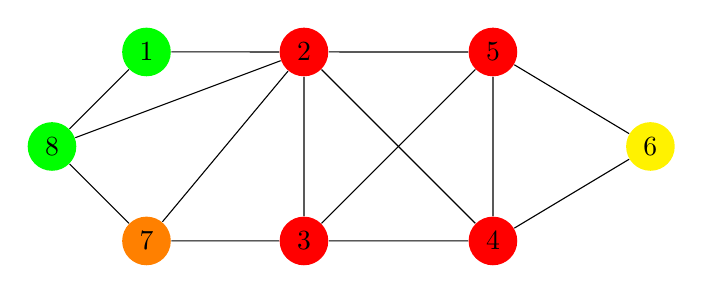
\begin{tikzpicture}
[scale=.8,every node/.style={circle,fill=blue!20}]
\node[fill=green] (n1) at (1.5,9) {1};
\node[fill=red] (n2) at (4,9) {2};
\node[fill=red] (n3) at (4,6) {3};
\node[fill=red] (n4) at (7,6) {4};
\node[fill=red] (n5) at (7,9) {5};
\node[fill=yellow] (n6) at (9.5,7.5) {6};
\node[fill=orange] (n7) at (1.5,6) {7};
\node[fill=green] (n8) at (0,7.5) {8};
\foreach \from/\to in {n1/n2,n2/n3,n2/n5,n3/n4,n5/n4,n5/n6,n4/n6,n3/n7,n7/n8,n1/n8,n2/n4,n3/n5,n2/n7,n2/n8}
\draw (\from) -- (\to);
\end{tikzpicture}

However, we can find that $\theta(G)$ is equal to 3 (smallest I could find):
\\
\\
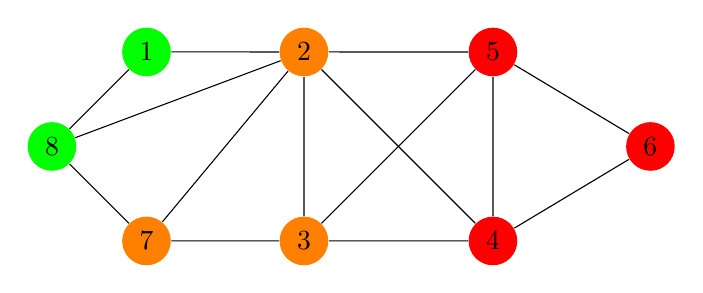
\begin{tikzpicture}
[scale=.8,every node/.style={circle,fill=blue!20}]
\node[fill=green] (n1) at (1.5,9) {1};
\node[fill=orange] (n2) at (4,9) {2};
\node[fill=orange] (n3) at (4,6) {3};
\node[fill=red] (n4) at (7,6) {4};
\node[fill=red] (n5) at (7,9) {5};
\node[fill=red] (n6) at (9.5,7.5) {6};
\node[fill=orange] (n7) at (1.5,6) {7};
\node[fill=green] (n8) at (0,7.5) {8};
\foreach \from/\to in {n1/n2,n2/n3,n2/n5,n3/n4,n5/n4,n5/n6,n4/n6,n3/n7,n7/n8,n1/n8,n2/n4,n3/n5,n2/n7,n2/n8}
\draw (\from) -- (\to);
\end{tikzpicture}

As well, the clique number, $\omega(G)$, is 4:
\\
\\
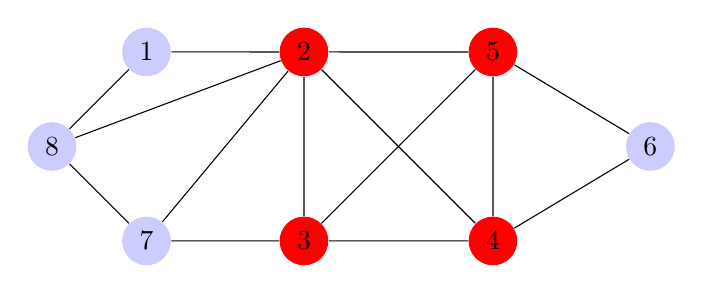
\begin{tikzpicture}
[scale=.8,every node/.style={circle,fill=blue!20}]
\node (n1) at (1.5,9) {1};
\node[fill=red] (n2) at (4,9) {2};
\node[fill=red] (n3) at (4,6) {3};
\node[fill=red] (n4) at (7,6) {4};
\node[fill=red] (n5) at (7,9) {5};
\node (n6) at (9.5,7.5) {6};
\node (n7) at (1.5,6) {7};
\node (n8) at (0,7.5) {8};
\foreach \from/\to in {n1/n2,n2/n3,n2/n5,n3/n4,n5/n4,n5/n6,n4/n6,n3/n7,n7/n8,n1/n8,n2/n4,n3/n5,n2/n7,n2/n8}
\draw (\from) -- (\to);
\end{tikzpicture}

\end{exmp}

\begin{definition}[Perfect Graph]
A graph G is perfect if $\chi(G) = \omega(G)$ for all induced subgraphs, H, of G.

\end{definition}

\subsubsection{Graphs with an Eigensharp decomposition by Stars}

\subsection{Other Bounds on Independence Number}

\section{Algorithm to Find Graphs Lacking a Tight Inertia Bound}

\subsection{Outline of Method}

\begin{definition}[Optimal Weight Matrix]
A weight matrix, $W$, of a graph, $G$, is optimal if
\begin{equation}
\alpha(G) = \min\{|G| - n_+(W),|G| - n_-(W)\}
\end{equation}
\end{definition}

\begin{exmp}
Consider the following graph, $G$, with corresponding weight matrix $W$:

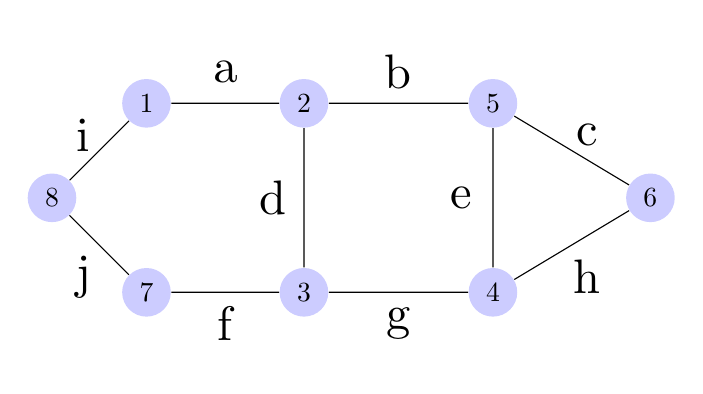
\begin{tikzpicture}
[scale=.8,every node/.style={circle,fill=blue!20}]
\node[scale=1.75,fill=white] (a) at (2.75,9.5) {a};
\node[scale=1.75,fill=white] (b) at (5.5,9.5) {b};
\node[scale=1.75,fill=white] (c) at (8.5,8.5) {c};
\node[scale=1.75,fill=white] (d) at (3.5,7.5) {d};
\node[scale=1.75,fill=white] (e) at (6.5,7.5) {e};
\node[scale=1.75,fill=white] (f) at (2.75,5.5) {f};
\node[scale=1.75,fill=white] (g) at (5.5,5.5) {g};
\node[scale=1.75,fill=white] (h) at (8.5,6.25) {h};
\node[scale=1.75,fill=white] (i) at (0.5,8.5) {i};
\node[scale=1.75,fill=white] (j) at (0.5,6.25) {j};
\node (n1) at (1.5,9) {1};
\node (n2) at (4,9) {2};
\node (n3) at (4,6) {3};
\node (n4) at (7,6) {4};
\node (n5) at (7,9) {5};
\node (n6) at (9.5,7.5) {6};
\node (n7) at (1.5,6) {7};
\node (n8) at (0,7.5) {8};
\foreach \from/\to in {n1/n2,n2/n3,n2/n5,n3/n4,n5/n4,n5/n6,n4/n6,n3/n7,n7/n8,n1/n8}
\draw (\from) -- (\to);
\end{tikzpicture}

$
\begin{bmatrix}
0 & a & 0 & 0 & 0 & 0 & 0 & i \\
a & 0 & d & 0 & b & 0 & 0 & 0\\
0 & d & 0 & g & 0 & 0 & f & 0 \\
0 & 0 & g & 0 & e & h & 0 & 0 \\
0 & b & 0 & e & 0 & c & 0 & 0 \\
0 & 0 & 0 & h & c & 0 & 0 & 0 \\
0 & 0 & f & 0 & 0 & 0 & 0 & j\\
i & 0 & 0 & 0 & 0 & 0 & j & 0\\
\end{bmatrix}
$
\\

We can see the independent number of $G$ is 3:

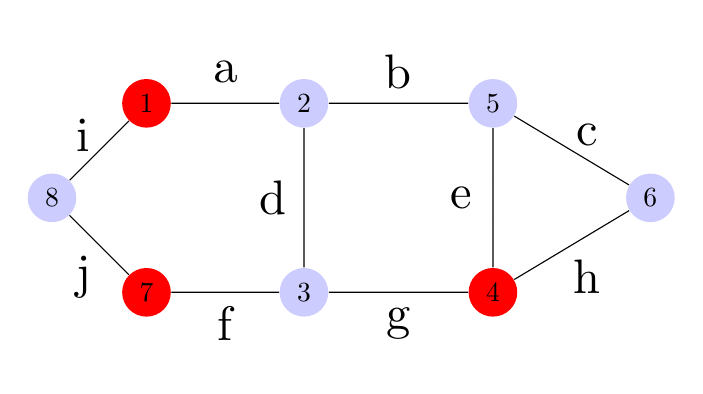
\begin{tikzpicture}
[scale=.8,every node/.style={circle,fill=blue!20}]
\node[scale=1.75,fill=white] (a) at (2.75,9.5) {a};
\node[scale=1.75,fill=white] (b) at (5.5,9.5) {b};
\node[scale=1.75,fill=white] (c) at (8.5,8.5) {c};
\node[scale=1.75,fill=white] (d) at (3.5,7.5) {d};
\node[scale=1.75,fill=white] (e) at (6.5,7.5) {e};
\node[scale=1.75,fill=white] (f) at (2.75,5.5) {f};
\node[scale=1.75,fill=white] (g) at (5.5,5.5) {g};
\node[scale=1.75,fill=white] (h) at (8.5,6.25) {h};
\node[scale=1.75,fill=white] (i) at (0.5,8.5) {i};
\node[scale=1.75,fill=white] (j) at (0.5,6.25) {j};
\node[fill=red] (n1) at (1.5,9) {1};
\node (n2) at (4,9) {2};
\node (n3) at (4,6) {3};
\node[fill=red] (n4) at (7,6) {4};
\node (n5) at (7,9) {5};
\node (n6) at (9.5,7.5) {6};
\node[fill=red] (n7) at (1.5,6) {7};
\node (n8) at (0,7.5) {8};
\foreach \from/\to in {n1/n2,n2/n3,n2/n5,n3/n4,n5/n4,n5/n6,n4/n6,n3/n7,n7/n8,n1/n8}
\draw (\from) -- (\to);
\end{tikzpicture}

Now, let G have the following weighting:

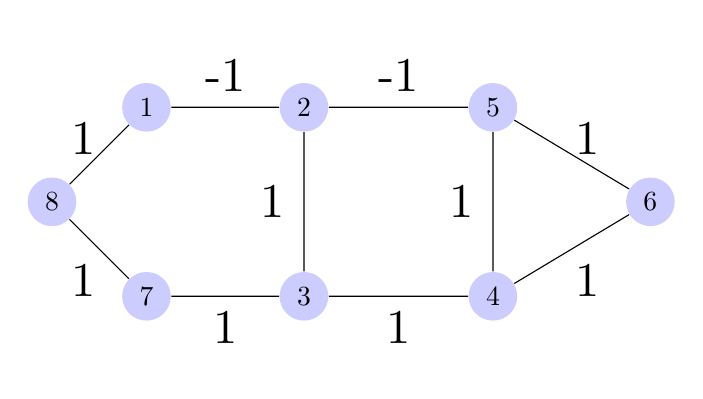
\begin{tikzpicture}
[scale=.8,every node/.style={circle,fill=blue!20}]
\node[scale=1.75,fill=white] (a) at (2.75,9.5) {-1};
\node[scale=1.75,fill=white] (b) at (5.5,9.5) {-1};
\node[scale=1.75,fill=white] (c) at (8.5,8.5) {1};
\node[scale=1.75,fill=white] (d) at (3.5,7.5) {1};
\node[scale=1.75,fill=white] (e) at (6.5,7.5) {1};
\node[scale=1.75,fill=white] (f) at (2.75,5.5) {1};
\node[scale=1.75,fill=white] (g) at (5.5,5.5) {1};
\node[scale=1.75,fill=white] (h) at (8.5,6.25) {1};
\node[scale=1.75,fill=white] (i) at (0.5,8.5) {1};
\node[scale=1.75,fill=white] (j) at (0.5,6.25) {1};
\node (n1) at (1.5,9) {1};
\node (n2) at (4,9) {2};
\node (n3) at (4,6) {3};
\node (n4) at (7,6) {4};
\node (n5) at (7,9) {5};
\node (n6) at (9.5,7.5) {6};
\node (n7) at (1.5,6) {7};
\node (n8) at (0,7.5) {8};
\foreach \from/\to in {n1/n2,n2/n3,n2/n5,n3/n4,n5/n4,n5/n6,n4/n6,n3/n7,n7/n8,n1/n8}
\draw (\from) -- (\to);
\end{tikzpicture}

$
\begin{bmatrix}
0 & -1 & 0 & 0 & 0 & 0 & 0 & 1 \\
-1 & 0 & 1 & 0 & -1 & 0 & 0 & 0\\
0 & 1 & 0 & 1 & 0 & 0 & 1 & 0 \\
0 & 0 & 1 & 0 & 1 & 1 & 0 & 0 \\
0 & -1 & 0 & 1 & 0 & 1 & 0 & 0 \\
0 & 0 & 0 & 1 & 1 & 0 & 0 & 0 \\
0 & 0 & 1 & 0 & 0 & 0 & 0 & 1\\
1 & 0 & 0 & 0 & 0 & 0 & 1 & 0\\
\end{bmatrix}
$
\\

Finding the eigenvalues of $W$, we find there are 3 positive eigenvalues and 5 negative eigenvalues. Thus, we see for this weight matrix we have:

\begin{equation}
\begin{split}
\alpha(G) & = \min\{|G| - n_+(W),|G| - n_-(W)\} \\
& = \min\{8 - 3,8 - 5\} \\
& = \min\{5,3\} \\
& = 3
\end{split}
\end{equation}

Therefore, this is an optimal weight matrix of G.

Now consider the following weighting for the same graph:

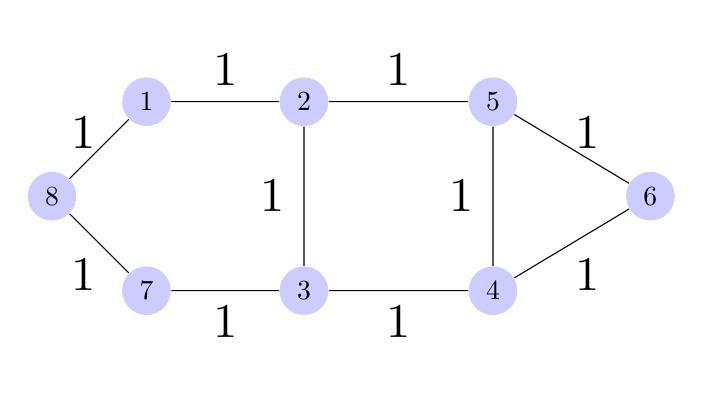
\begin{tikzpicture}
[scale=.8,every node/.style={circle,fill=blue!20}]
\node[scale=1.75,fill=white] (a) at (2.75,9.5) {1};
\node[scale=1.75,fill=white] (b) at (5.5,9.5) {1};
\node[scale=1.75,fill=white] (c) at (8.5,8.5) {1};
\node[scale=1.75,fill=white] (d) at (3.5,7.5) {1};
\node[scale=1.75,fill=white] (e) at (6.5,7.5) {1};
\node[scale=1.75,fill=white] (f) at (2.75,5.5) {1};
\node[scale=1.75,fill=white] (g) at (5.5,5.5) {1};
\node[scale=1.75,fill=white] (h) at (8.5,6.25) {1};
\node[scale=1.75,fill=white] (i) at (0.5,8.5) {1};
\node[scale=1.75,fill=white] (j) at (0.5,6.25) {1};
\node (n1) at (1.5,9) {1};
\node (n2) at (4,9) {2};
\node (n3) at (4,6) {3};
\node (n4) at (7,6) {4};
\node (n5) at (7,9) {5};
\node (n6) at (9.5,7.5) {6};
\node (n7) at (1.5,6) {7};
\node (n8) at (0,7.5) {8};
\foreach \from/\to in {n1/n2,n2/n3,n2/n5,n3/n4,n5/n4,n5/n6,n4/n6,n3/n7,n7/n8,n1/n8}
\draw (\from) -- (\to);
\end{tikzpicture}

$
\begin{bmatrix}
0 & 1 & 0 & 0 & 0 & 0 & 0 & 1 \\
1 & 0 & 1 & 0 & 1 & 0 & 0 & 0\\
0 & 1 & 0 & 1 & 0 & 0 & 1 & 0 \\
0 & 0 & 1 & 0 & 1 & 1 & 0 & 0 \\
0 & 1 & 0 & 1 & 0 & 1 & 0 & 0 \\
0 & 0 & 0 & 1 & 1 & 0 & 0 & 0 \\
0 & 0 & 1 & 0 & 0 & 0 & 0 & 1\\
1 & 0 & 0 & 0 & 0 & 0 & 1 & 0\\
\end{bmatrix}
$
\\

Finding the eigenvalues of this weight matrix, we find there are 4 positive eigenvalues and 4 negative eigenvalues. Thus, we see we get:

\begin{equation}
\begin{split}
\alpha(G) = 3 & \neq \min\{|G| - n_+(W),|G| - n_-(W)\} \\
& = \min\{8 - 4,8 - 4\} \\
& = \min\{4,4\} \\
& = 4
\end{split}
\end{equation}

Therefore, we see that the previous weighting was not optimal for G.
\end{exmp}

\begin{lemma}
If a graph, $G$, with weight matrix $W$, has two induced subgraphs, $S_1$ and $S_2$, such that $S_1$ has $\alpha(G)+1$ positive eigenvalues under the weighting of $W$, and $S_2$ has $\alpha(G)+1$ negative eigenvalues under the weighting of $W$, then $W$ is not optimal
\end{lemma}

\begin{proof}



\end{proof}

\subsection{Preliminary Tests to Determine if the Graph may be Suitable}

\subsubsection{Test for $\alpha-$Critical}

\begin{definition}[$\bm{\alpha-}$Critical]
A graph, G, is $\alpha-$critical if $\alpha(G) < \alpha(G-e)$ for all edges e.
\end{definition}

\begin{exmp}
Consider the following graph G:

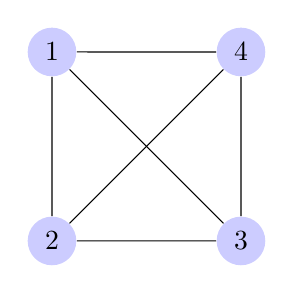
\begin{tikzpicture}
[scale=.8,every node/.style={circle,fill=blue!20}]
\node (n1) at (4,9) {1};
\node (n2) at (4,6) {2};
\node (n3) at (7,6) {3};
\node (n4) at (7,9) {4};
\foreach \from/\to in {n1/n2,n1/n3,n1/n4,n2/n3,n2/n4,n3/n4}
\draw (\from) -- (\to);
\end{tikzpicture}

we see that $\alpha(G) = 1$. But since this graph is complete, we see that if we delete any edge, we can get an independent set of size 2 by making the set include the two vertices that were connected by the edge we deleted. For example:

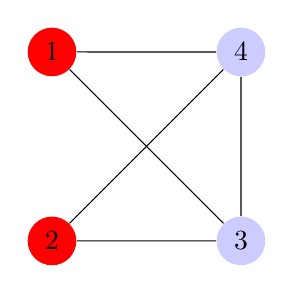
\begin{tikzpicture}
[scale=.8,every node/.style={circle,fill=blue!20}]
\node[fill = red] (n1) at (4,9) {1};
\node[fill = red] (n2) at (4,6) {2};
\node (n3) at (7,6) {3};
\node (n4) at (7,9) {4};
\foreach \from/\to in {n1/n3,n1/n4,n2/n3,n2/n4,n3/n4}
\draw (\from) -- (\to);
\end{tikzpicture}

Thus, G is $\alpha-$critical.
\end{exmp}

\begin{lemma}
\label{alpha}
If G is $\alpha-$critical, and $W$ an optimal weight matrix of G, then $w_{i,j} \neq$ 0 for all $i,j \in E(G)$
\end{lemma} 
\begin{proof}
Assume for the sake of contradiction, that for some $i,j \in E(G)$, we have $w_{i,j} = 0$. Then, we know $\alpha(G-e_{i,j}) > \alpha(G)$ because G is $\alpha-$critical. Thus:

$\alpha(G) < \alpha(G-e_{i,j}) \leq \min\{|G| - n_+(W),|G| - n_-(W)\}$

Thus, we see that the inertia bound is not tight for G, so W is not an optimal weight matrix of G, which is a contradiction.
\end{proof}

Due to the complexity of needing to consider edges that could potentially be zero in the weight matrix, it is easier to consider graphs that are restricted to only non-zero edge weights in its optimal weight matrix. Thus, it makes sense to only consider $\alpha-$critical graphs, because of Lemma \ref{alpha} ensuring that all $\alpha-$critical graphs have non-zero weight matrices.

\subsubsection{Determining Each Triangle Must Have the Same Sign}


\subsection{Graphs Currently Found}

\renewcommand{\thempfootnote}{\arabic{mpfootnote}}
\begin{center}
\begin{minipage}{\textwidth}
\begin{tabular}{ |p{1cm}|p{1.5cm}|p{0.5cm}|p{1.5cm}|p{2.7cm}|p{2cm}| } 
 \hline
 Graph & Vertices & $\alpha$ & Degree & Circulant & Strongly Regular\\ 
 \hline
 \footnote{Otr@PKoE?T\_iOoOG\_dg\_m} & 16 & 4 & 5 & No & No\\
 \hline
 \footnote{O$\sim\sim$em]uj[vmsZTUrfFwN$\sim$} & 16 & 2 & 10 & No & (16,10,6,6) \\
 \hline
 \footnote{P\}qtSeLUbaKeQZJabfGmmG$\sim$G} & 17 &  3 & 8 & [1,2,4,8] & (17,8,3,4)\\
 \hline
 \footnote{R\}ecZ@OH?o\`W@gOWcI\_\`p?hkHL?GuG} & 19 & 4 & 6 & [1,7,8] & No \\
 \hline
 \footnote{S$\sim\sim$vVjjve\}vmxymlG$\sim$Oi$\sim$Qm\{jfxjNw\{z\{} & 20 & 2 & 13 & No & No \\
 \hline
 \footnote{S$\sim\sim$vnZjvUtvimj`$\sim$nibtTP\}[ffwk$\sim$wR$\sim$\{} & 20 & 2 & 13 & [1,3,4,7,8,9,10] & No\\
 \hline
 \footnote{Uv$\sim$LnbgfeDShP\textbackslash{}G\}HuXmePrSemapSxqJWG$\vert$ZCVhw} & 22 & 3 & 11 & [1,2,3,5,10,11] & No\\
 \hline
 \footnote{Wunneyzx$\sim$W]OwBPfcroK$\sim$S\{OlogtIoyPlPFMIIjWPUvaGu$\sim$} & 24 & 3 & 12 & No & No \\
 \hline
 \footnote{WvrlvjZj$\sim$c\textbackslash{}\_wBTRcroK$\sim$K\{HLpGtPo[ikpImQHrWaUn`Cv\^{}} & 24 & 3 & 12 & No & No \\
 \hline
 \footnote{WvvdtIJpB\_c[LEHPiH?PsE\_GAsWKcwBXhGDgOFXWIBV@CZT} & 24 & 4 & 9 & No & No\\
 \hline
 \footnote{W\}mKmIbqD\_JJMMBYa]\_\{??ucC\{YKeHKXPadVXOmqQbqEDMp} & 24 & 4 & 10 & [1,2,4,8,9] & No\\
 \hline
 \footnote{W\}nS$\vert$QeoOq\_nWS]?KcPQUPDgU@\_TBG\_ug@ei?jCgCwY\_?J$\sim$} & 24 & 4 & 9 & No & No\\
 \hline
 \footnote{W\}\}VNbMtdyWkic?zg]gevHT\_TfGo$\sim$bPK$\vert$xHkJJMolozdq\textbackslash{}s} & 24 & 3 & 12 & No & No \\
 \hline
 \footnote{W\}$\sim$SvAbp@IcjDgEaj?@BKPCgBbXP@oCz?BLdE@KwGu[?EFZ} & 24 & 4 & 9 & No & No\\
 \hline
 \footnote{W$\sim$nELU\textbackslash{}`aKkXTJ]?@cGUB@KgBSX?wG\_sS`DUCGyWO`\}?@M\^{}} & 24 & 4 & 9 & No & No \\
 \hline
 \footnote{W$\sim\sim\sim$vnnv$\vert$$\sim$\}gzH\}`za$\vert$J\^{}ef$\vert\sim$wBJNisn[bn\^{}@\^{}nwez$\sim$`V\^{}$\sim$} & 24 & 2 & 16 & No & No\\
 \hline
 \footnote{W$\sim\sim\sim$vnn\{vT\{nvFnFo\^{}\}$\sim$Dnw\textbackslash{}\{\^{}AF$\vert$hFz[YZ$\sim$DT$\sim$wX\^{}$\sim$n\{B$\sim$} & 24 & 2 & 16 & No & No\\
 \hline
 \footnote{W$\sim\sim\sim$vnn\{vXyjqnnFs\^{}\}$\sim$Knw\textbackslash{}[\^{}QF$\vert$hiz[iznCt$\sim$wX\^{}$\sim$n\{B$\sim$} & 24 & 2 & 16 & [1,2,3,4,6,7,8,10] & No\\
 \hline
 \footnote{W$\sim\sim\sim$vvu$\vert$\^{}\textbackslash{}\textbackslash{}jvivTvtTyj\_$\sim\vert$\}ibyiiF\}[b\{$\sim$C\{$\sim$wU\^{}$\sim$\_f$\sim\sim$} & 24 & 2 & 16 & No & No\\
 \hline
\end{tabular}
\end{minipage}
\end{center}

\section{Other Useful Information}

\subsection{Cayley Graphs}
\begin{definition}[Cayley Graph]


\end{definition}




\bibliographystyle{plain}
\bibliography{mybib}

\end{document}



